\chapter{Authentication Testing}

	Authentication is the act of establishing or confirming something (or someone) as authentic, 
	that is, that claims made by or about the thing are true. Authenticating an object may
	mean confirming its provenance, whereas authenticating a person often consists of verifying her 
	identity. Authentication depends upon one or more authentication factors. In computer security,
	authentication is the process of attempting to verify the digital identity of the sender of a
	communication. A common example of such a process is the logon process. Testing the authentication 
	schema means understanding how the authentication process works and using that information to 
	circumvent the authentication mechanism.

\clearpage

\section{Credentials Transport Over An Encrypted Channel}
	Testing for credentials transport means to verify that the user's authentication data are transferred 
	via an encrypted channel to avoid being intercepted by malicious users. The analysis focuses simply 
	on trying to understand if the data travels unencrypted from the web browser to the server, or if the 
	web application takes the appropriate security measures using a protocol like HTTPS. The HTTPS protocol 
	is built on TLS/SSL to encrypt the data that is transmitted and to ensure that user is being sent towards
	the desired site. Clearly, the fact that traffic is encrypted does not necessarily mean that it's
	completely safe. The security also depends on the encryption algorithm used and the robustness of the 
	keys that the application is using, but this particular topic will not be addressed in this section. 

	Nowadays, the most common example of this issue is the login page of a web application. In order to 
	log into a web site, usually, the user has to fill a simple form that transmits the inserted data with 
	the POST method. What is less obvious is that this data can be passed using the HTTP protocol, that 
	means in a non-secure way, or using HTTPS, which encrypts the data.

	It is strongly suggested to use the POST method instead og GET. This is because when the GET method 
	is used, the url that it requests is easily available from, for example, the server logs exposing 
	your sensitive data to information leakage.

		\begin{figure}[H]
			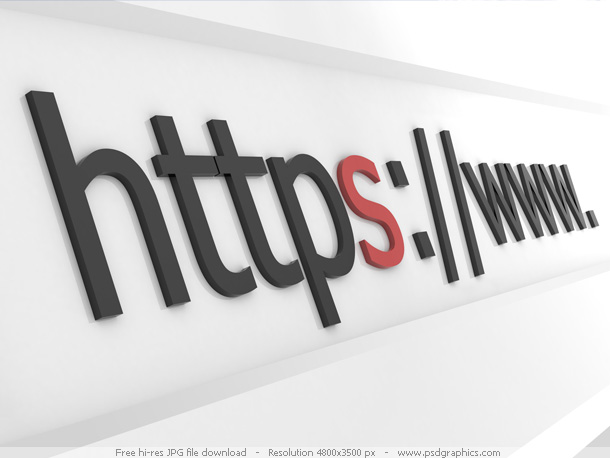
\includegraphics[scale=0.4]{pics/https.jpg}
		\end{figure}

\section{User Enumeration}

	The scope of this test is to verify if it is possible to collect a set of valid usernames by 
	nteracting with the authentication mechanism of the application. This test will be useful for the 
	brute force testing, in which we verify if, given a valid username, it is possible to find the
	corresponding password. Often, web applications reveal when a username exists on system, either 
	as a consequence of a misconfiguration or as a design decision. For example, sometimes, when we 
	submit wrong credentials, we receive a message that states that either the username is present 
	on the system or the provided password is wrong. 

	In some cases, we receive a message that reveals if the provided credentials are wrong because an 
	invalid username or an invalid password was used. Sometimes, we can enumerate the existing users 
	by sending a username and an empty password.

	{\bf Testing for nonexisting username} \\
	Generally the application should respond with the same error message and length to the different 
	wrong requests. If you notice that the responses are not the same, you should investigate and find 
	out the key that creates a difference between the 2 responses. For example:

	{\color{red} Client request: Valid user/wrong password -- Server answer:'The password is not correct'}

	{\color{red} Client request: Wrong user/wrong password -- Server answer:'User not recognized'}

	{\bf URI Probing} \\
	Sometimes a web server responds differently if it receives a request for an existing directory or 
	not. For instance in some portals every user is associated with a directory, if we try to access 
	an existing directory we could receive a web server error. A very common error that we can receive 
	from web server is:

	\begin{itemize}
		\item {\bf 403 Forbidden error code}
		\item {\bf 404 Not found error code}
		\item http://www.foo.com/account1 - we receive from web server: 403 Forbidden
		\item http://www.foo.com/account2 - we receive from web server: 404 file Not Found
	\end{itemize}

	In first case the user exists, but we cannot view the web page, in second case instead the user
	“account2” doesn’t exist. Collecting this information we can enumerate the users.

	{\bf Guessing Users} \\
	In some cases the userIDs are created with specific policies of administrator or company. 
	Other possibilities are userIDs associated with credit card numbers, or in general a numbers 
	with a pattern. For example we can view a user with a userID created in sequential order:

	{\color{blue} CN000100, CN000101, .....}

\section{Guessable User Account}

	Today's web applications typically run on popular open source or commercial software that is 
	installed on servers and requires configuration or customization by the server administrator. 
	In addition, most of today's hardware appliances, i.e., network routers and database servers, 
	offer web-based configuration or administrative interfaces.

	In addition, it is typical to find generic accounts, left over from testing or administration,
	that use common usernames and passwords and are left enabled in the application and its 
	infrastructure. These default username and password combinations are widely known by penetration 
	testers and malicious attackers, who can use them to gain access to various types of custom, 
	open source, or commercial applications.

	In addition, weak password policy enforcements seen in many applications allow users to sign up 
	using easy to guess usernames and passwords, and may also not allow password changes to be 
	undertaken.

	{\bf The root cause of this problem can be identified as:}
		\begin{itemize}
			\item Inexperienced IT personnel, who are unaware of the importance of changing default 
			passwords on installed infrastructure components.
			\item Programmers who leave backdoors to easily access and test their application and 
			later forget to remove them.
			\item Application administrators and users that choose an easy username and password 
			for themselves.
			\item Applications with built-in, non-removable default accounts with a pre-set username 
			and password.
			\item Applications which leak information as to the validity of usernames during either
			authentication attempts, password resets, or account signup.
		\end{itemize}
	
	An additional problem stems from the use of blank passwords, which are simply the result of a lack 
	of security awareness or a desire to simplify administration.

	Note that the application being tested may have an account lockout, and multiple password guess 
	attempts with a known username may cause the account to be locked. If it is possible to lock the
	administrator account, it may be troublesome for the system administrator to reset it

	{\bf Approach for testing:}
	\begin{itemize}
		\item Try the following usernames - "admin", "administrator", "root", "system", "guest", "operator",
		or "super". These are popular among system administrators and are often used. In addition try an 
		empty password or one of the following "password", "pass123", "password123", "admin", or "guest" 
		with the above accounts or any other enumerated accounts. 
		\item Application administrative users are often named after the application or organization. 
		\item When performing a test for a customer, attempt using names of contacts you have received 
		as usernames with any common passwords.
		\item Viewing the User Registration page may help determine the expected format and length of 
		the application usernames and passwords.
		\item Attempt using all the above usernames with blank passwords.
		\item Review the page source and javascript either through a proxy or by viewing the source. 
		Look for any references to users and passwords in the source.
		\item Look for account names and passwords written in comments in the source code. Also look 
		in backup directories, etc for source code that may contain comments of interest.
		\item Try to extrapolate from the application how usernames are generated. For example, 
		can a user create their own username or does the system create an account for the user based 
		on some personal information or a predictable sequence? 
	\end{itemize}


\clearpage
\section{Brute Force}
	Brute-forcing consists of systematically enumerating all possible candidates for the solution 
	and checking whether each candidate satisfies the problem's statement. Here is several types of
	bruteforce attacks:

	{\bf Dictionary Attack} \\
	Dictionary-based attacks consist of automated scripts and tools that will try to guess username 
	and passwords from a dictionary file. A dictionary file can be tuned and compiled to cover words 
	probably used by the owner of the account that a malicious user is going to attack. The attacker 
	can gather information (via active/passive reconnaissance, competitive intelligence, dumpster 
	diving, social engineering) to understand the user, or build a list of all unique words available 
	on the website.

	{\bf Search Attacks} \\
	Search attacks will try to cover all possible combinations of a given character set and a given 
	password length range. This kind of attack is very slow because the space of possible candidates 
	is quite big. 

	{\bf Rule-based search attacks} \\
	To increase combination space coverage without slowing too much of the process it's suggested to 
	create good rules to generate candidates. For example "John the Ripper" can generate password 
	variations from part of the username or modify through a preconfigured mask words in the input 
	(e.g. 1st round "pen" -- 2nd round "p3n" -- 3rd round "p3np3n").

	\begin{figure}[H]
		\centering
		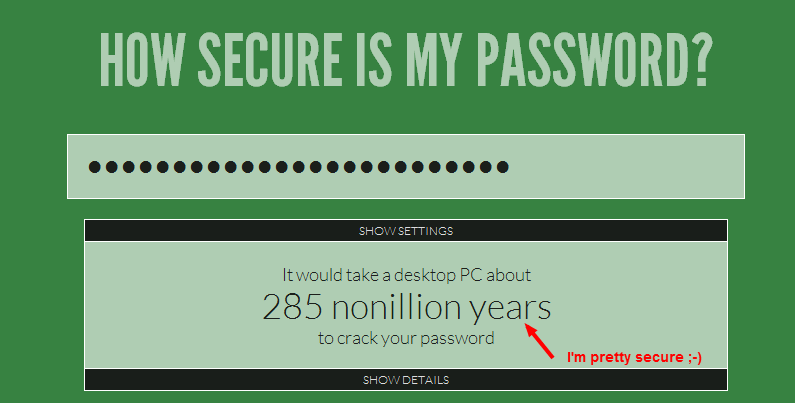
\includegraphics[scale=0.1]{pics/bruteforce2.png}
	\end{figure}

	\clearpage
	Nowadays, a common attacks are based on Rainbow Tables, a special type of lookup table used in 
	recovering the plaintext password from a ciphertext generated by a one-way hash.
	Tables are specific to the hash function they were created for e.g., MD5 tables can only crack MD5 
	hashes. The more powerful RainbowCrack program was later developed that can generate and use rainbow
	tables for a variety of character sets and hashing algorithms, including LM hash, MD5, SHA1, etc.

	\begin{figure}[H]
		
\includegraphics[width=\textwidth]{pics/rainbow.png}
	\end{figure}




\section{Bypassing Authentication Schema}

	While most applications require authentication for gaining access to private information or 
	to execute tasks, not every authentication method is able to provide adequate security.
	There are several methods to bypass the authentication schema in use by a web application:
		\begin{itemize}
			\item Direct page request (forced browsing)
			\item Parameter Modification
			\item Session ID Prediction
			\item SQL Injection
		\end{itemize}


\section{Vulnerable remember password and reset}
	Most web applications allow users to reset their password if they have forgotten it, usually 
	by sending them a password reset email and/or by asking them to answer one or more 
	"security questions".

	A great majority of web applications provide a way for users to recover (or reset) their password 
	in case they have forgotten it. The exact procedure varies heavily among different applications, 
	also depending on the required level of security, but the approach is always to use an alternate 
	way of verifying the identity of the user. One of the simplest (and most common) approaches is 
	to ask the user for his/her e-mail address, and send the old password (or a new one) to that
	address. This scheme is based on the assumption that the user's email has not been compromised 
	and that is secure enough for this goal.

	Alternatively (or in addition to that), the application could ask the user to answer one or more 
	"secret questions", which are usually chosen by the user among a set of possible ones. 
	The security of this scheme lies in the ability to provide a way for someone to identify themselves 
	to the system with answers to questions that are not easily answerable via personal information 
	lookups. As an example, a very insecure question would be “your mother’s maiden name” since that 
	is a piece of information that an attacker could find out without much effort. An example of a 
	better question would be “favorite grade-school teacher” since this would be a much more difficult 
	topic to research about a person whose identity may otherwise already be stolen.

	Another common feature that applications use to provide users a convenience, is to cache the 
	password locally in the browser (on the client machine) and having it 'pre-typed' in all 
	subsequent accesses. While this feature can be perceived as extremely friendly for the average 
	user, at the same time it introduces a flaw, as the user account becomes easily accessible
	to anyone that uses the same machine account.

\section{Browser Cache Management}
	In this phase, we check that the logout function is properly implemented, and that it is not 
	possible to “reuse” a session after logout. We also check that the application automatically 
	logs out a user when that user has been idle for a certain amount of time, and that no sensitive 
	data remains stored in the browser cache.

	{\bf Logout function:} \\
	The first step is to test the presence of the logout function. Check that the application provides 
	a logout button and that this button is present and well visible on all pages that require  
	authentication. A logout button that is not clearly visible, or that is present only on certain 
	pages, poses a security risk, as the user might forget to use it at the end of his/her session.
	The second step consists in checking what happens to the session tokens when the logout function 
	is invoked. For instance, when cookies are used a proper behavior is to erase all session cookies, 
	by issuing a new Set-Cookie directive that sets their value to a non-valid one (e.g.: “NULL” or 
	some equivalent value) and, if the cookie is persistent, setting its expiration date in the past, 
	which tells the browser to discard the cookie. The first (and simplest) test at this point consists 
	of logging out and then hitting the 'back' button of the browser, to check whether we are still
	authenticated. If we are, it means that the logout function has been implemented insecurely, and 
	that the logout function does not destroy the session IDs. It should be noted that this test only 
	applies to session cookies, and that a persistent cookie that only stores data about some minor 
	user preferences (e.g.: site appearance) and that is not deleted when the user logs out is not 
	to be considered a security risk.

	{\bf Timeout logout:} \\
	The most appropriate logout time should be a right balance between security (shorter logout time) 
	and usability (longer logout time) and heavily depends on the criticality of the data handled by 
	the application. A 60 minute logout time for a public forum can be acceptable, but such a long time 
	would be way too much in a home banking application.

	{\bf Cached pages:} \\
	Logging out from an application obviously does not clear the browser cache of any sensitive 
	information that might have been stored. Therefore, another test that is to be performed is to 
	check that our application does not leak any critical data into the browser cache. In order to 
	do that, we can use WebScarab and search through the server responses that belong to our session,
	checking that for every page that contains sensitive information the server instructed the browser 
	not to cache any data. Such a directive can be issued in the HTTP response headers. 

	{\bf As a general rule, we need to check that:}
		\begin{itemize}
			\item The logout function effectively destroys all session token, or at least renders 
			them unusable
			\item The server performs proper checks on the session state, disallowing an attacker 
			to replay some previous token.
			\item A timeout is enforced and it is properly checked by the server. If the server 
			uses an expiration time that is read from a session token that is sent by the client, 
			the token must be cryptographically protected.
		\end{itemize}

\section{Captcha}
	{\bf CAPTCHA ("Completely Automated Public Turing test to tell Computers and Humans Apart")} is a
	type of challenge-response test used by many web applications to ensure that the response is not
	generated by a computer. CAPTCHA implementations are often vulnerable to various kinds of attacks 
	even if the generated CAPTCHA is unbreakable. This section will help you to identify these kinds 
	of attacks.

	Although CAPTCHA is not an authentication control, its use can be very efficient against:
		\begin{itemize}
			\item enumeration attacks (login, registration or password reset forms are often vulnerable 
			to enumeration attacks - without CAPTCHA the attacker can gain valid usernames, phone numbers 
			or any other sensitive information in a short time)
			\item automated sending of many GET/POST requests in a short time where it is undesirable 
			(e.g., SMS/MMS/email flooding), CAPTCHA provides a rate limiting function
			\item automated creation/using of the account that should be used only by humans 
			(e.g., creating webmail accounts, stop spamming)
			\item automated posting to blogs, forums and wikis, whether as a result of commercial 
			promotion, or harassment and vandalism
			\item any automated attacks that massively gain or misuse sensitive information from 
			the application
		\end{itemize}

	These vulnerabilities are quite common in many CAPTCHA implementations:
	\begin{itemize}
		\item generated image CAPTCHA is weak, this can be identified (without any complex computer
		recognition systems) only by a simple comparison with already broken CAPTCHAs
		\item generated CAPTCHA questions have a very limited set of possible answers
		\item the value of decoded CAPTCHA is sent by the client (as a GET parameter or as a 
		hidden field of POST form). This value is often: {\bf 1)} encrypted by simple algorithm and 
		can be easily decrypted by observing of multiple decoded CAPTCHA values. 
		{\bf 2)} hashed by a weak hash function (e.g., MD5) that can be broken using a rainbow 
		table 
		\item possibility of replay attacks:
			{\bf 1)} the application does not keep track of what ID of CAPTCHA image is sent to 
			the user. Therefore, the attacker can simply obtain an appropriate CAPTCHA image and 
			its ID, solve it, and send the value of the decoded CAPTCHA with its corresponding ID 
			(the ID of a CAPTCHA could be a hash of the decoded CAPTCHA or any unique identifier)
			{\bf 2)} the application does not destroy the session when the correct phrase is entered 
			- by reusing the session ID of a known CAPTCHA it is possible to bypass CAPTCHA protected 
			page
	\end{itemize}


\section{Multiple Factors Authentication}

	“Multiple Factors Authentication System” (MFAS) is a critical task for the Penetration tester.
	Generally the aim of a two factor authentication system is to enhance the strength of the 
	authentication process. This goal is achieved by checking an additional factor, or “something 
	you have” as well as “something you know”, making sure that the user holds a hardware device of 
	some kind in addition to the password. The hardware device provided to the user may be able to
	communicate directly and independently with the authentication infrastructure using an additional
	communication channel; this particular feature is something known as “separation of channels”.
	Bruce Schneier in 2005 observed that some years ago “the threats were all passive: eavesdropping 
	and offline password guessing. Today, the threats are more active: phishing and Trojan horses”. 
	Actually the common threats that a MFAS in a Web environment should correctly address include:
		\begin{enumerate}
			\item Weak Credentials (Credentials Password guessing and Password Bruteforcing attacks)
			\item Credential Theft (Phishing, Eavesdropping, MITM e.g. Banking from compromised network)
			\item Session based attacks (Session Riding, Session Fixation)
			\item Trojan and Malware attacks (Banking from compromised clients)
			\item Password Reuse (Using the same password for different purposes or operations, 
			e.g. different transactions)
		\end{enumerate}

	The typical IT professional’s advise is: “If you are not happy with your current
	authentication solution, just add another authentication factor and it will be all right”.

	MFAS solutions add “something you have” to the authentication process. This component is usually a:
		\begin{itemize}
			\item One-time password (OTP) generator token.
			\item Grid Card, Scratch Card, or any information that only the legitimate user is 
			supposed to have in his wallet
			\item Crypto devices like USB tokens or smart cards.
			\item Randomly generated OTPs transmitted through a GSM SMS messages.
		\end{itemize}

\section{Race Conditions}

	A race condition is a flaw that produces an unexpected result when the timing of actions impact 
	other actions. An example may be seen on a multithreaded application where actions are being 
	performed on the same data. Race conditions, by their very nature, are difficult to test for.

	Race conditions may occur when a process is critically or unexpectedly dependent on the sequence 
	or timings of other events. In a web application environment, where multiple requests can be 
	processed at a given time, developers may leave concurrency to be handled by the framework, 
	server, or programming language. The following simplified example illustrates a potential 
	concurrency problem in a transactional web application and relates to a joint savings account 
	in which both users (threads) are logged into the same account and attempting a transfer.

	{\bf \color{red} Account A has 100 credits}

	{\bf \color{blue} Account B has 100 credits}

	Both User 1 and User 2 want to transfer 10 credits from Account A to Account B. If the 
	transaction was correct the outcome should be:

	{\bf \color{red} Account A has 80 credits}

	{\bf \color{blue} Account B has 120 credits}

	However, due to concurrency issues, the following result could be obtained:

	{\bf User 1 checks the value of Account A (=100 credits)}

	{\bf User 2 checks the value of Account A (=100 credits)}

	{\bf User 2 takes 10 credits from Account A (=90 credits) and put it in Account B (=110 credits)}

	{\bf User 1 takes 10 credits from Account A (Still believed to contain 100 credits) 
	(=90 credits) and puts it into Account B (=120 credits).}

	{\bf \color{red} Result: Account A has 90 credits}
	
	{\bf \color{blue} Account B has 120 credits}

	However, testing can be focused on specific transactional areas of the application, where 
	time-of-read to time-of-use of specific data variables could be adversely affected by concurrency 
	issues.


